

\chapter{Modelling of a rotating free-floating object dynamic interactions with a mass moving on its surface}
\label{ch:Stability study}
TOCHANGE!! purpose In this chapter is designing mass changes as control method one needs to establish the effect of changes of mass distributioon on a rotating free floating rotational motion and determine if there are and if so under what kind of conditions the motion of a mass at the surface of a free floating objects will imact its rotational motions
delpoyment of structure on frre floating object

define the stability of the rotational motion of the obejct???

System definition and model: The system is composed of an undeformable rotating object and a modular robot made out of identical spherical modules. The robots moves and deploys itself at the surface of the object by maintianing contact at all time. As the rotational motion is the only focus of this study, the system is considered to be isolated.
The best way to model is to use 

\section{Introductory illustration the Yo-Yo despin mechanism}
\label{Introductory illustration the Yo-Yo despin mechanism}




Write..\gls{ghc}
Write..\gls{ghc}.

\section{Introductory illustration the Yo-Yo despin mechanism}
\label{Introductory illustration the Yo-Yo despin mechanism}

\subsection{Yo-Yo despin mechanism description}
\label{Yo-Yo despin mechanism description}

%\begin{figure}[h]
%	\begin{center}
%		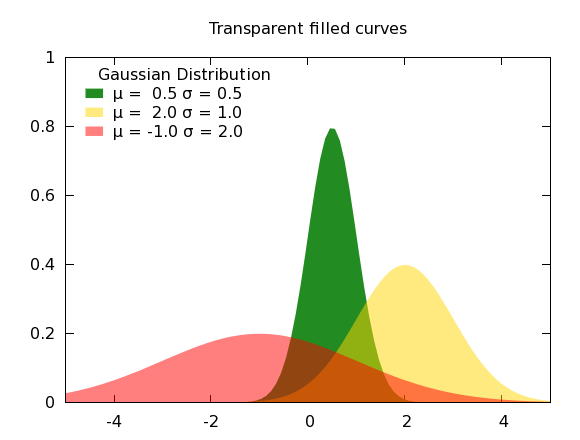
\includegraphics [width=12cm]{Figures/Background/pic.png}
%		\caption{Figure Caption.}
%		\label{fig:Yo-Yo despin mechanism seen in its plane of rotation}
%	\end{center}
%\end{figure} 



\section{System modelling}
\label{System modelling}
The Yo-Yo despin mechanism is discrete in order to generalise the robot and object were considered as a deformablee continuum where a rigid part (the object) would interact with a deformable part (the robot). The general model can be discrtized in order to accomodate the modular structure of the robot and simplify the dynamic equations of the system.

the model is directly derived from [PAPER]
\subsection{Continuous model}
\label{Continuous model}

As per [PAPER] the continuous model is the following: IN THE BODY FRAME
\begin{center}
\begin{equation*} 
\end{equation*}
\end{center}\
$[\bf I]\cdot \dot{\overrightarrow{\bf \Omega}} + \overrightarrow{\bf \Omega} \wedge [\bf I]\cdot \overrightarrow{\bf \Omega} + 2[\bf J]\cdot \overrightarrow{\bf \Omega}+ $

${d\over dt}{\int_{m}[(\overrightarrow{\bf \Psi} \otimes \overrightarrow{\bf x})\cdot \overrightarrow{\bf x} - (\overrightarrow{\bf x}\otimes\overrightarrow{\bf x})\cdot \overrightarrow{\bf \Psi}]dm}$



$+ \int_{m}{[(\overrightarrow{\bf x}\otimes \dot{\overrightarrow{\bf x''_{0}}}) - (\dot{\overrightarrow{\bf x''_{0}}}\otimes \overrightarrow{\bf x}) ]\cdot \overrightarrow{\bf \Psi}dm}$

$+\overrightarrow{\bf \Omega}\cdot \int_{m}{[(\overrightarrow{\bf x}\otimes \overrightarrow{\bf x})\wedge \overrightarrow{\bf \Psi}+((\overrightarrow{\bf x}\otimes \overrightarrow{\bf x})\wedge \overrightarrow{\bf \Psi})^{T}]dm}$

$\int_{m}(\overrightarrow{\bf x}\wedge \ddot{\overrightarrow{\bf x''_{0}}})
=\overrightarrow{\bf M}_{Body} + \overrightarrow{\bf M}_{Stresses}$




with $\overrightarrow{\bf \Omega}=\overrightarrow{\bf \Omega(t)}$ rigid body rotation constant over the continuum but depenmdent on time, $\overrightarrow{\bf \Psi}=\overrightarrow{\bf \Psi}(\overrightarrow{\bf x},t)$ dependent on the position whitihn the continuum and the time. 

$[\bf J]= \int_{m}{[(\overrightarrow{\bf v''_{0}} \cdot \overrightarrow{\bf x})[\bf 1] - \overrightarrow{\bf v''_{0}}\otimes \overrightarrow{\bf x}]dm}$.

Although model of a continuum, the interaction between mass(module) and the object does not constitute a stress hence $\overrightarrow{\bf M}_{Stresses}=\overrightarrow{\bf 0}$. Moreover the system is isolated so $\overrightarrow{\bf M}_{Body}=\overrightarrow{\bf 0}$.

\subsection{Discrete point mass model}
\label{Discrete point mass model}
For the purpose of studying the stability of the sytem will be studied with one moving mass along the surface of the object. This leads to the following discrete model:

$[\bf I]\cdot \dot{\overrightarrow{\bf \Omega}} + \overrightarrow{\bf \Omega} \wedge [\bf I]\cdot \overrightarrow{\bf \Omega}=$

$- 2m \big [(\dot{\overrightarrow{\bf x''_{0}}} \cdot \overrightarrow{\bf x})[\bf 1] - \dot{\overrightarrow{\bf x''_{0}}}\otimes \overrightarrow{\bf x}\big ]\cdot \overrightarrow{\bf \Omega}$

$-m \bigg [ \big [(\overrightarrow{\bf x} \cdot \overrightarrow{\bf x})[\bf 1]-(\overrightarrow{\bf x} \otimes \overrightarrow{\bf x}) \big] \cdot \dot{\overrightarrow{\bf \Psi}} + \big [2(\overrightarrow{\bf x}\cdot \dot{\overrightarrow{\bf x}})[\bf 1]-(\dot{\overrightarrow{\bf x}} \otimes \overrightarrow{\bf x})-(\overrightarrow{\bf x} \otimes \dot{\overrightarrow{\bf x}}) \big ]\cdot \overrightarrow{\bf \Psi} \bigg ]$

$-m{\big [(\overrightarrow{\bf x}\otimes \dot{\overrightarrow{\bf x''_{0}}}) - (\dot{\overrightarrow{\bf x''_{0}}}\otimes \overrightarrow{\bf x}) \big ]\cdot \overrightarrow{\bf \Psi}}$

$-m {\big [(\overrightarrow{\bf x}\otimes \overrightarrow{\bf x})\wedge \overrightarrow{\bf \Psi}+((\overrightarrow{\bf x}\otimes \overrightarrow{\bf x})\wedge \overrightarrow{\bf \Psi})^{T}\big ] \cdot \overrightarrow{\bf \Omega}}$

$-m(\overrightarrow{\bf x}\wedge \ddot{\overrightarrow{\bf x''_{0}}})$


Since the mass is bound to the surface the system is holonomic. Using the spherical cooordinates the relative kinematic properties of the mass with respect to the object can be expressed only with $\phi$ and $\theta$. The relative rotational speed and acceleration are respectively $\overrightarrow{\bf \Psi}=()$ and  $\dot \dot{\overrightarrow{\bf\Psi}}=()$ as projected in the body frame.

The point hypothesis there is no additional rotation of the mass due to its following the surface (SEE DIAGRAM TO DRAW p58 my notebook). The local body coordiante system of the mass $[O'']$ can be considrerd to be the local shperical coordiante system. This leads to a the discrete model in body coordinate that will be used for our stability study:
$[\bf I]\cdot \dot{\overrightarrow{\bf \Omega}} + \overrightarrow{\bf \Omega} \wedge [\bf I]\cdot \overrightarrow{\bf \Omega}=$




 \glspl{pe}.

\section{System equilibria}
\label{System equilibrian}

In [BOOK]  

Write.. \gls{pe}.

Write.. \glspl{pe}.

\section{Hamiltonian Lagrange formulation}
\label{Hamiltonian Lagrange formulation}

Write.. \gls{pe}.

Write.. \glspl{pe}.

%\begin{figure}[h]
% \begin{center}
% 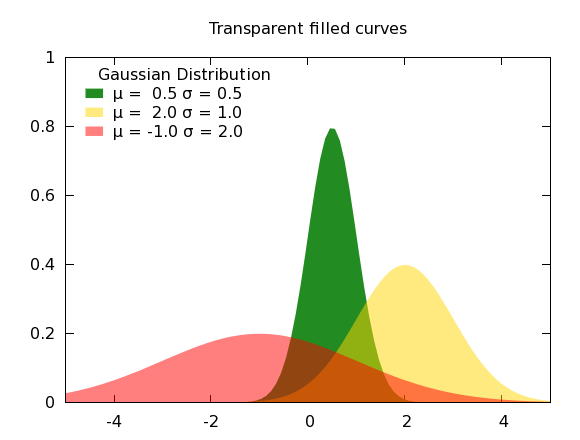
\includegraphics [width=12cm]{Figures/Background/pic.png}
% \caption{Figure Caption.}
% \label{fig:label}
%\end{center}
%\end{figure} 
%
%\cite{gum, ghc-smp}
%
%\subsection{Subsection}
%
%\begin{table}[h]
%\begin{center}
%\begin{tabular}{c c c c} % centered columns (4 columns)
%\hline\hline %inserts double horizontal lines
%Case & Method\#1 & Method\#2 & Method\#3 \\ [0.5ex] % inserts table 
%%heading
%\hline % inserts single horizontal line
%1 & 50 & 837 & 970 \\ % inserting body of the table
%2 & 47 & 877 & 230 \\
%3 & 31 & 25 & 415 \\
%4 & 35 & 144 & 2356 \\
%5 & 45 & 300 & 556 \\ [1ex] % [1ex] adds vertical space
%\hline %inserts single line
%\end{tabular}\caption{Table Caption}
%\label{tab:lable}
%\end{center}
%\end{table}
%
%
%\subsubsection{Subsubsection}